\section{Verteilungen der betrachteten Spalten der Evaluation}

\begin{figure}[h!]
\centering
	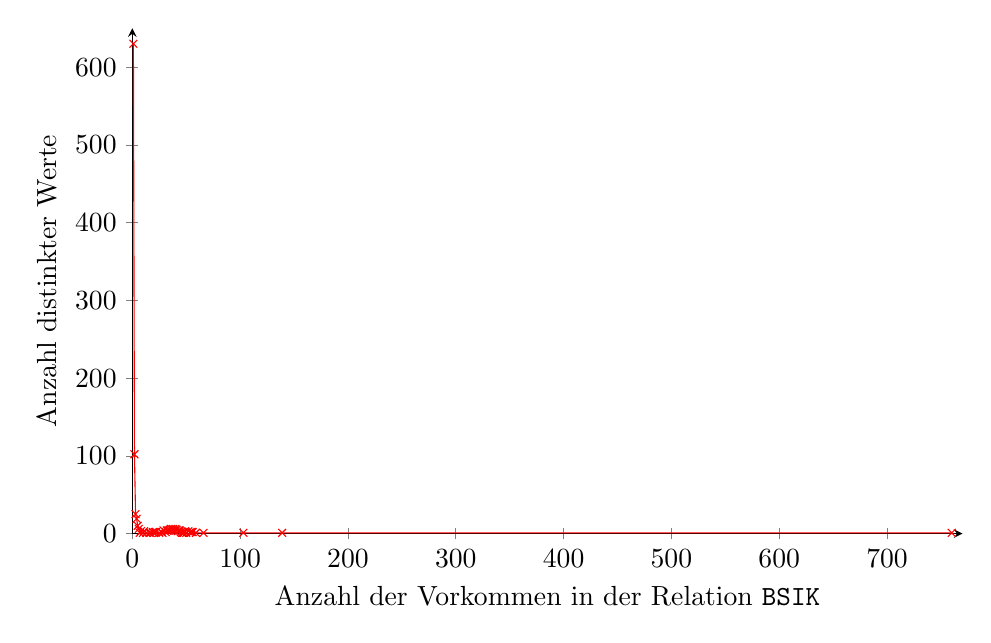
\begin{tikzpicture}
		\begin{axis}[
				axis lines=left,
				width  = 1*\textwidth,
				height  = 8cm,
				ylabel={Anzahl distinkter Werte},
				xlabel={Anzahl der Vorkommen in der Relation \texttt{BSIK}},
				ymin=0.0,
				xmin=0.0,
				ymax=650.0,
				xmax=770.0,
				]
				\addplot[color=red,mark=x] coordinates {
					(1,630)
					(2,102)
					(3,25)
					(4,19)
					(5,10)
					(6,6)
					(7,1)
					(8,3)
					(10,1)
					(11,3)
					(13,1)
					(16,1)
					(17,1)
					(19,2)
					(20,1)
					(21,2)
					(22,2)
					(25,1)
					(27,2)
					(28,1)
					(29,4)
					(31,2)
					(32,4)
					(33,4)
					(34,4)
					(35,5)
					(36,6)
					(37,5)
					(38,6)
					(39,4)
					(40,6)
					(41,5)
					(42,3)
					(43,4)
					(44,4)
					(45,2)
					(46,1)
					(47,1)
					(48,1)
					(49,3)
					(50,1)
					(52,3)
					(54,2)
					(55,2)
					(56,2)
					(59,1)
					(66,1)
					(103,1)
					(139,1)
					(760,1)
				};
		\end{axis}
	\end{tikzpicture}
	\caption{Verteilung der distinkten Werte in der Spalte \texttt{BUDAT}}
	\label{fig:budatverteilung}
\end{figure}


\begin{figure}[h!]
\centering
	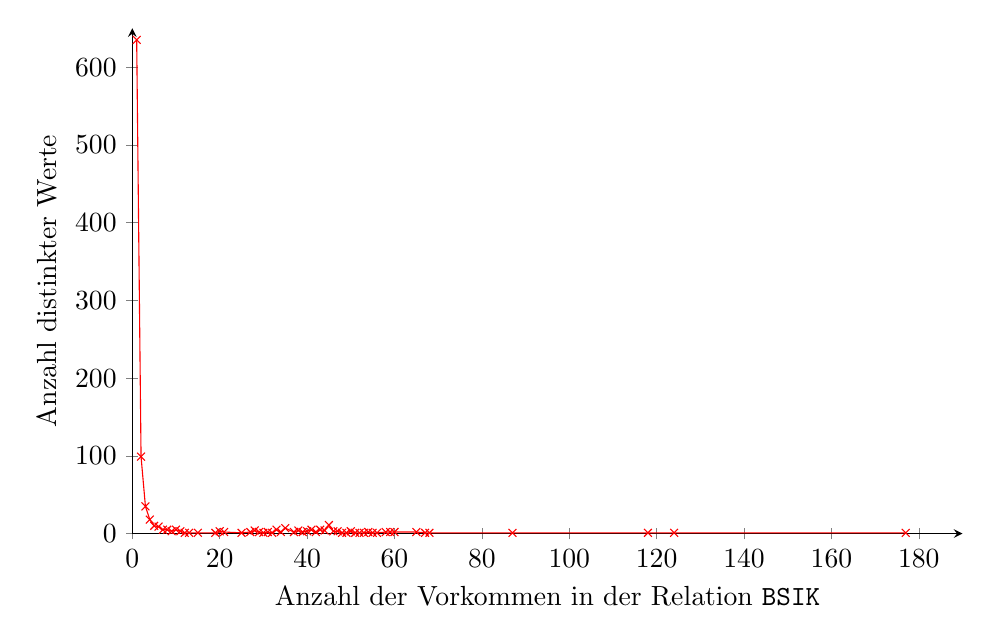
\begin{tikzpicture}
		\begin{axis}[
				axis lines=left,
				width  = 1*\textwidth,
				height  = 8cm,
				ylabel={Anzahl distinkter Werte},
				xlabel={Anzahl der Vorkommen in der Relation \texttt{BSIK}},
				ymin=0.0,
				xmin=0.0,
				ymax=650.0,
				xmax=190.0,
				]
				\addplot[color=red,mark=x] coordinates {
					(1,635)
					(2,99)
					(3,35)
					(4,18)
					(5,10)
					(6,9)
					(7,5)
					(8,5)
					(9,3)
					(10,5)
					(11,3)
					(12,1)
					(13,1)
					(15,1)
					(19,1)
					(20,3)
					(21,2)
					(25,1)
					(27,2)
					(28,4)
					(29,2)
					(30,1)
					(31,2)
					(32,1)
					(33,5)
					(34,2)
					(35,7)
					(37,2)
					(38,4)
					(39,2)
					(40,3)
					(41,5)
					(42,2)
					(43,5)
					(44,4)
					(45,11)
					(46,3)
					(47,3)
					(48,1)
					(49,1)
					(50,3)
					(51,1)
					(52,1)
					(53,1)
					(54,2)
					(55,1)
					(56,1)
					(58,2)
					(59,2)
					(60,2)
					(65,2)
					(67,1)
					(68,1)
					(87,1)
					(118,1)
					(124,1)
					(177,1)
				};
		\end{axis}
	\end{tikzpicture}
	\caption{Verteilung der distinkten Werte in der Spalte \texttt{BLDAT}}
	\label{fig:bldatverteilung}
\end{figure}


\begin{figure}[h!]
\centering
	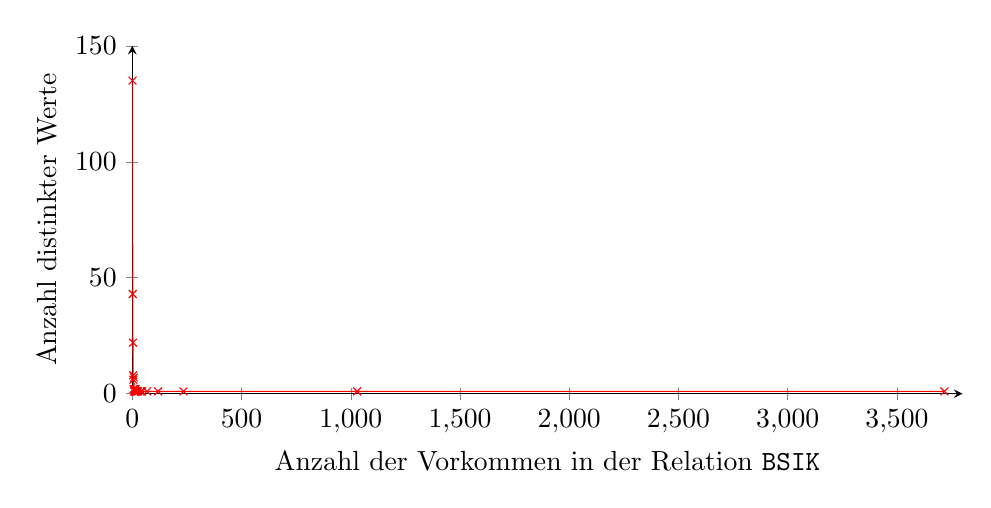
\begin{tikzpicture}
		\begin{axis}[
				axis lines=left,
				width  = 1*\textwidth,
				height  = 6cm,
				ylabel={Anzahl distinkter Werte},
				xlabel={Anzahl der Vorkommen in der Relation \texttt{BSIK}},
				ymin=0.0,
				xmin=0.0,
				ymax=150.0,
				xmax=3800.0,
				]
				\addplot[color=red,mark=x] coordinates {
					(1,135)
					(2,43)
					(3,22)
					(4,8)
					(5,6)
					(6,2)
					(7,7)
					(8,2)
					(9,1)
					(10,1)
					(11,1)
					(12,2)
					(13,1)
					(14,1)
					(15,1)
					(16,2)
					(19,1)
					(20,1)
					(23,1)
					(27,1)
					(41,1)
					(42,1)
					(45,1)
					(67,1)
					(118,1)
					(234,1)
					(1029,1)
					(3717,1)
				};
		\end{axis}
	\end{tikzpicture}
	\caption{Verteilung der distinkten Werte in der Spalte \texttt{LIFNR}}
	\label{fig:lifnrverteilung}
\end{figure}


\begin{figure}[h!]
\centering
	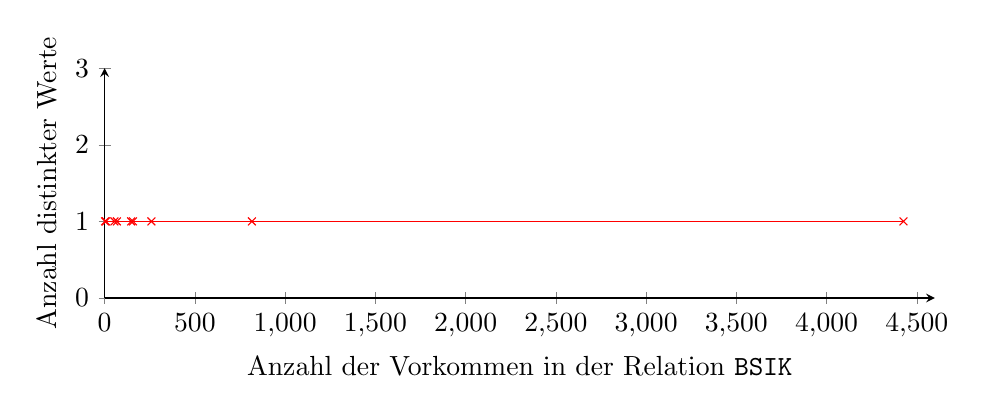
\begin{tikzpicture}
		\begin{axis}[
				axis lines=left,
				width  = 1*\textwidth,
				height  = 4.5cm,
				ylabel={Anzahl distinkter Werte},
				xlabel={Anzahl der Vorkommen in der Relation \texttt{BSIK}},
				ymin=0.0,
				xmin=0.0,
				ymax=3.0,
				xmax=4600.0,
				]
				\addplot[color=red,mark=x] coordinates {
					(2,1)
					(7,1)
					(54,1)
					(68,1)
					(147,1)
					(157,1)
					(259,1)
					(816,1)
					(4426,1)
				};
		\end{axis}
	\end{tikzpicture}
	\caption{Verteilung der distinkten Werte in der Spalte \texttt{BUKRS}}
	\label{fig:bukrsverteilung}
\end{figure}

\begin{figure}[h!]
\centering
	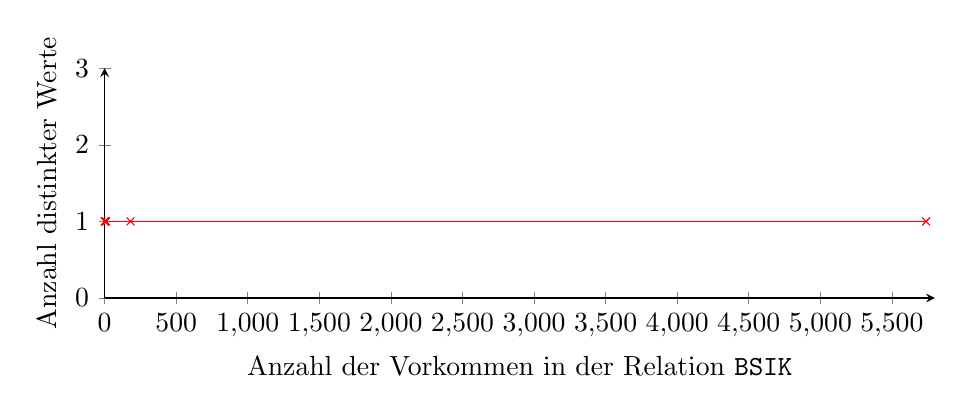
\begin{tikzpicture}
		\begin{axis}[
				axis lines=left,
				width  = 1*\textwidth,
				height  = 4.5cm,
				ylabel={Anzahl distinkter Werte},
				xlabel={Anzahl der Vorkommen in der Relation \texttt{BSIK}},
				ymin=0.0,
				xmin=0.0,
				ymax=3.0,
				xmax=5800.0,
				]
				\addplot[color=red,mark=x] coordinates {
					(1,1)
					(2,1)
					(3,1)
					(10,1)
					(181,1)
					(5739,1)
				};
		\end{axis}
	\end{tikzpicture}
	\caption{Verteilung der distinkten Werte in der Spalte \texttt{ZLSCH}}
	\label{fig:zlschverteilung}
\end{figure}